\documentclass[t, pdftex]{beamer}  
%Use Cockrell School Theme.  Optional department name.  Must %ecape, i.e. use 
%backslash, to preserve spaces.  The default is ``Cockrell School of Engineering''
%\usetheme[]{Cockrell}                 
%\usetheme[dept=Aerospace\ Engineering\ and\ Engineering\ Mechanics]{cockrell}                 
%\usetheme[dept=Biomedical\ Engineering]{cockrell}                 
%\usetheme[dept=Chemical\ Engineering]{cockrell}                 
%\usetheme[dept=Civil,\ Architectural\ and\ Environmental\ Engineering]{cockrell}                 
\usetheme[dept=Electrical\ and\ Computer\ Engineering]{Cockrell}                 
%\usetheme[dept=Mechanical\ Engineering]{cockrell}                 
%\usetheme[dept=Materials\ Science\ and\ Engineering]{cockrell}                 
%\usetheme[dept=Petroleum\ and\ Geosystems\ Engineering]{cockrell}                 

% Add preamble packages here
%\usepackage{etex}
%\usepackage[bigfiles]{media9}
\usepackage{graphicx}
\graphicspath{{../figs/}}
\usepackage{caption}

\usepackage{listings,multicol}
\definecolor{ForestGreen}{rgb}{0.13,0.55,0.13}
\lstset{
    language         = Promela,
    basicstyle       = \ttfamily,
    keywordstyle     = \bfseries\color{blue},
    stringstyle      = \color{magenta},
    commentstyle     = \color{ForestGreen},
    showstringspaces = false,
}

%Enable cancelto in math
\usepackage{cancel}
\renewcommand{\CancelColor}{\color{utorange}}

%Add bibliography file location for citiation
% \bibliography{example.bib}


\title{Verifying Distributed Algorithms}
\subtitle{in Promela}
\author{Eric Crosson \\ Nhan Do \\ Stormy Mauldin \\ Daniel Officewala}
\institute{EE 360P}
\date{\today}


\begin{document}

%Creates title frame from title, subtitle, author, institute, and date above
\titleframe

%Supports table of contents
\frame{\frametitle{Outline}\tableofcontents}

%Section commands will define what's shown in TOC

%First frame
\section{Introducing Promela}
\begin{frame}
    \frametitle{What are Spin and Promela?}
    Spin is a multi-threaded software verification tool that supports the high-level language Promela to specify models of systems.
    \begin{itemize}
      \item Promela allows the user to create parallel programs that define processes, message channels, and variables.
      \item From the promela program, Spin can then verify various system correctness properties as well as user-defined properties
    \end{itemize}
\end{frame}

\section{Dining Philosophers}
\begin{frame}[c]
  \frametitle{Dining Philosophers}
  \begin{multicols}{2}
    \textbf{Most Philosophers}
    \begin{itemize}
      \item Want to eat:
      \begin{itemize}
        \item Get left fork (or wait)
        \item Get right fork (or wait)
      \end{itemize}
      \item After eating:
      \begin{itemize}
        \item Release both forks
        \item Contemplate life until hungry
      \end{itemize}
    \end{itemize}
    \columnbreak
    \textbf{One "Special" Philosopher}
    \begin{itemize}
      \item Want to eat:
      \begin{itemize}
        \item Get left fork (or wait)
        \item Get right fork (if fail, release \textit{both} forks)
      \end{itemize}
      \item After eating:
      \begin{itemize}
        \item Release both forks
        \item Contemplate life until hungry
      \end{itemize}
    \end{itemize}
  \end{multicols}
\end{frame}

\begin{frame}[c]
  \frametitle{Dining Philosopher Analysis}
  \begin{multicols}{2}
    \begin{itemize}
      \item \textbf{Mutually Exclusive}
      \begin{itemize}
        \item A philospher must acquire both shared forks before eating
      \end{itemize}
      \item \textbf{Deadlock}
      \begin{itemize}
        \item The one special philosopher will always surrender both forks, allowing someone else to start eating.
      \end{itemize}
      \item \textbf{Starvation}
      \begin{itemize}
        \item The special philosopher always surrenders forks in case of conflict. May never get a change to eat.
      \end{itemize}
    \end{itemize}
    \columnbreak
    \begin{figure}
      \begin{minipage}{.5\textwidth}
        \centering
        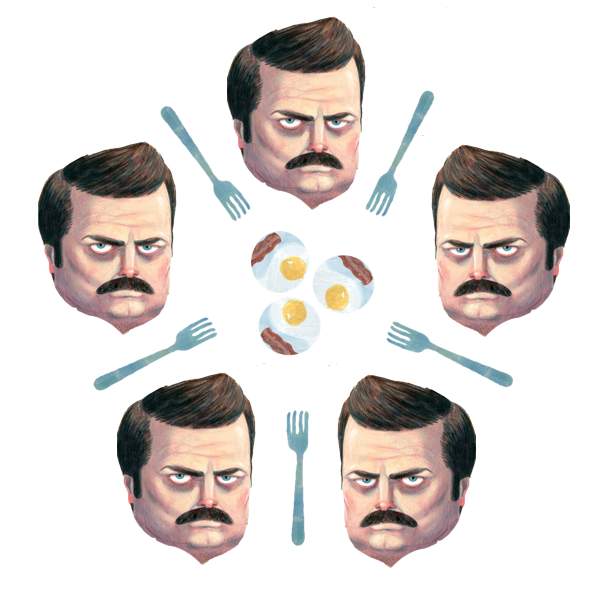
\includegraphics[scale=.20]{DiningPhilosophers}
        \captionof{figure}{Hungry, hungry philosophers}
      \end{minipage}
    \end{figure}
  \end{multicols}
\end{frame}



\section{Token Ring}
\begin{frame}[c]
    \frametitle{Token Ring Algorithm}
    % \TeX\ \cite{knuth1989} and \LaTeX\ \cite{lamport1986} are great for equations
    \begin{itemize}
		\item Simple and easily scalable
		 \begin{itemize}
          \item Pass token around ring of processes
          \item Only processes with token can enter CS
		  \item No Starvation
        \end{itemize}
    \end{itemize}
	
	
 \begin{figure}
	 \begin{minipage}{.5\textwidth}
      \centering
      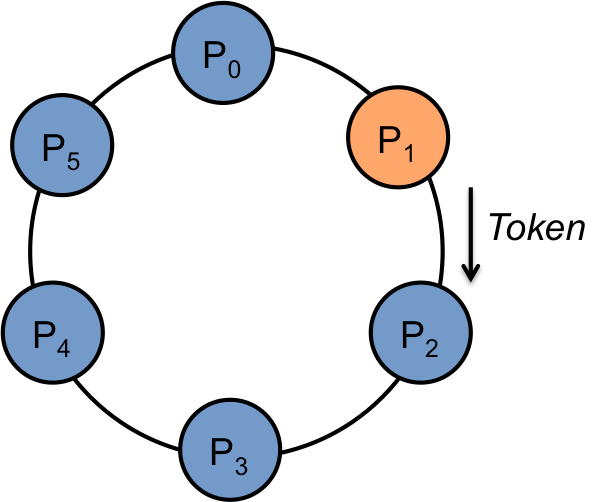
\includegraphics[scale=.30]{tokenring}
      \captionof{figure}{Token Ring Algorithm}
      \label{fig:Token Ring}
    \end{minipage}
\end{figure}
	
\end{frame}

\begin{frame}
	\frametitle{Token Ring Implementation}
	  \begin{multicols*}{3}
    \lstinputlisting[language=Promela, basicstyle=\tiny]{../figs/tokenring.pml}
  \end{multicols*}
\end{frame}



\section{Lamport's}
\begin{frame}[c]
    \frametitle{Lamport's}
    % \TeX\ \cite{knuth1989} and \LaTeX\ \cite{lamport1986} are great for equations
    \begin{block}{An equation block}
        \[ \vec{F} = m \vec{a} \]
    \end{block}
    \begin{itemize}
        \item Second instance of citations use short citation hyperlinked to original.
    \end{itemize}
\end{frame}

\section{Szymanski's}
\begin{frame}[c]
    \frametitle{Szymanski's Algorithm}
    \begin{itemize}
      \item Extension of Lamport's
        \begin{itemize}
          \item satisfies linear wait
          \item three booleans per process
        \end{itemize}
      \item Extension of Lamport's
    \end{itemize}
  % PRO POINTS: make your own charts here, don't be a scrub
  \begin{figure}
    \centering
    \begin{minipage}{.5\textwidth}
      \centering
      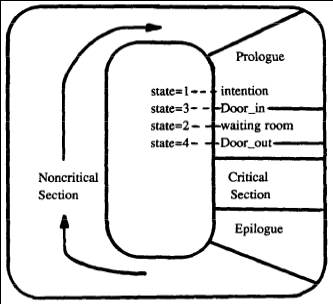
\includegraphics[scale=.3]{szymanskis_carosel}
      \captionof{figure}{Szymanski's Algorithm}
      \label{fig:szymanskis_carosel}
    \end{minipage}%
    \begin{minipage}{.5\textwidth}
      \centering
      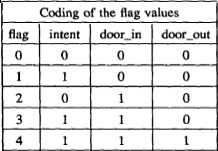
\includegraphics[scale=.61]{szymanskis_booleans}
      \captionof{figure}{State-tracking booleans}
      \label{fig:szymanskis_booleans}
    \end{minipage}
  \end{figure}
\end{frame}

\begin{frame}
  \frametitle{Szymanski's Implementation}
  \begin{multicols*}{3}
    \lstinputlisting[language=Promela, basicstyle=\tiny]{../figs/szymanski.pml}
  \end{multicols*}
\end{frame}

\begin{frame}
  \frametitle{Szymanski's Analysis}
  
\end{frame}

\section{Questions}
\begin{frame}[c]
    \frametitle{Questions}  % verbally, say ``What are your questions?'' 
    % \TeX\ \cite{knuth1989} and \LaTeX\ \cite{lamport1986} are great for equations
    \begin{itemize}
        \item English mothafucka, do you speak it?
    \end{itemize}
\end{frame}


% This command is causing problems
% I am not sure what we're missing out on by not having it.
%\lastframe%
\end{document}
